\section{Linear Regression \& Regularization}
\begin{frame}{Linear Regression}
    \begin{columns}[c]
        \begin{column}{0.55\textwidth}
            We start with the simplest assumption: \\
            The target $y$ is a \textbf{linear combination} of the input features.
            
            % \vspace{1em}
            $$ \hat{y} = w_0 + w_1 x_1 + w_2 x_2 + \dots + w_d x_d $$
            
            \vspace{1em}
            \textbf{The Components:}
            \begin{itemize}
                \item $\hat{y}$: predicted value
                \item $x_1, \dots, x_d$: the input features.
                \item $w_1, \dots, w_d$: the weights. How much each feature matters.
                \item $w_0$: the bias (Intercept). 
                
            \end{itemize}
        \end{column}

       \begin{column}{0.45\textwidth}
            \centering
            \begin{tikzpicture}[scale=0.7]
                \draw[->] (0,0) -- (5,0) node[right] {$x$};
                \draw[->] (0,0) -- (0,4) node[above] {$y$};
                % Points
                \foreach \x/\y in {1/1, 2/1.5, 3/3, 4/3.5} \filldraw[black] (\x,\y) circle (2pt);
                % Line
                \draw[blue, thick] (0,0.5) -- (5,4) node[right] {$\mathbf{X}\mathbf{w}$};
                % Residuals
                \draw[dashed, red] (3,3) -- (3,2.6);
            \end{tikzpicture}
        \end{column}
    \end{columns}
\end{frame}

\begin{frame}{Linear Regression}
    \begin{columns}[c]
        \begin{column}{0.55\textwidth}
            We start with the simplest assumption: \\
            The target $y$ is a \textbf{linear combination} of the input features.
            
            % \vspace{1em}
            $$ \hat{y} = w_0 + w_1 x_1 + w_2 x_2 + \dots + w_d x_d $$
            
            \vspace{1em}
            \textbf{The Components:}
            \begin{itemize}
                \item $\hat{y}$: predicted value
                \item $x_1, \dots, x_d$: the input features.
                \item $w_1, \dots, w_d$: the weights. How much each feature matters.
                \item $w_0$: the bias (Intercept). 
                
            \end{itemize}
            
        \end{column}

       \begin{column}{0.45\textwidth}
            \centering
            \begin{tikzpicture}[scale=0.7]
                \draw[->] (0,0) -- (5,0) node[right] {$x$};
                \draw[->] (0,0) -- (0,4) node[above] {$y$};
                % Points
                \foreach \x/\y in {1/1, 2/1.5, 3/3, 4/3.5} \filldraw[black] (\x,\y) circle (2pt);
                % Line
                \draw[blue, thick] (0,0.5) -- (5,4) node[right] {$\mathbf{X}\mathbf{w}$};
                % Residuals
                \draw[dashed, red] (3,3) -- (3,2.6);
            \end{tikzpicture}
        \end{column}
    \end{columns}
    Writing long sums ($\sum$) is tedious. We use Linear Algebra to represent Linear Regression in matrices notation.
\end{frame}

% --- Slide 2: Vectorization ---
\begin{frame}{Translating to Vectors (Vectorization)}
    % \vspace{1em}
    \textbf{Step 1: The Bias Trick:}
    We add a "dummy" feature $x_0 = 1$ to the input so we have each weight multiplied by a $x$ feature.
    $$ \hat{y} = w_0(1) + w_1 x_1 + \dots + w_d x_d $$
    
    % \vspace{1em}
    \textbf{Step 2: Vector Notation (For one sample):} We rewrite this equation in a vector dot product form:
    $$ \hat{y} = \begin{bmatrix} w_0 & w_1 & \dots & w_d \end{bmatrix} \cdot \begin{bmatrix} 1 \\ x_1 \\ \vdots \\ x_d \end{bmatrix} = \mathbf{w}^T \mathbf{x} $$

    \textbf{Step 3: Matrix Notation (For all data):} For $N$ samples, prediction becomes a simple Matrix-Vector multiplication:
        $$ \mathbf{\hat{y}} = \mathbf{X}\mathbf{w} $$

\end{frame}

% --- Slide 3: The Objective ---
\begin{frame}{Finding the Best Line}
    Now we have the equation. But how do we choose the best $\mathbf{w}$?
    \pause
    \\ We need the loss and the optimizer!
    \pause
    
    \vspace{1em}
    Let's wrap our model in the Mean Squared Error:
        $$ J(\mathbf{w}) = \frac{1}{N} ||\mathbf{X}\mathbf{w} - \mathbf{y}||^2_2 $$

    \pause
    \vspace{1em}
    \centering
    Now, how do we find the $\mathbf{w}$ that minimizes this $J(\mathbf{w})$?
    \pause
    
    \vspace{1em}
    \begin{columns}[c]
        \begin{column}{0.45\textwidth}
            \centering
            \textbf{Option A: Analytical}\\
            (Solve for zero gradient)
        \end{column}
        \begin{column}{0.1\textwidth}
            \centering \textbf{OR}
        \end{column}
        \begin{column}{0.45\textwidth}
            \centering
            \textbf{Option B: Iterative}\\
            (Gradient Descent)
        \end{column}
    \end{columns}
\end{frame}

% --- Slide 4: Normal Equation ---
\begin{frame}{Method A: The Normal Equation}
    For linear models, MSE is \textbf{convex}. \textbf{Q:} What does that tell you? \pause \textit{Guaranteed Global Minimum!}. \\
    \pause
    \textbf{Step 1: The Gradient} Derived via Chain Rule:
    $$ \nabla J(\mathbf{w}) = \frac{2}{N} \mathbf{X}^T(\mathbf{X}\mathbf{w} - \mathbf{y}) $$ 
    \pause    
    \textbf{Step 2: Set to Zero}
    $$ \mathbf{X}^T\mathbf{X}\mathbf{w} - \mathbf{X}^T\mathbf{y} = 0 $$
    $$ \mathbf{X}^T\mathbf{X}\mathbf{w} = \mathbf{X}^T\mathbf{y} $$

    \pause
    
    \textbf{Step 3: Solve for $\mathbf{w}$}
    Multiply both sides by inverse $(\mathbf{X}^T\mathbf{X})^{-1}$:
    \begin{tcolorbox}[colback=blue!5, width=0.45\linewidth, center]
        \centering\textbf{The Normal Equation}
        $$\mathbf{w} = (\mathbf{X}^T\mathbf{X})^{-1} \mathbf{X}^T \mathbf{y}$$
    \end{tcolorbox}
    \small \textit{Cons: Inverting large matrices is very slow $(O(d^3))$. Doesn't work if $X$ is singular.}
\end{frame}

% --- Slide 5: Gradient Descent ---
\begin{frame}{Method B: Gradient Descent}
    Instead of jumping to the solution, we take small steps.
    
    \textbf{Step 1: Calculate Gradient}
    Derived via Chain Rule:
    $$ \nabla J(\mathbf{w}) = \frac{2}{N} \mathbf{X}^T(\mathbf{X}\mathbf{w} - \mathbf{y}) $$ 
    
    \textbf{Step 2: Update Rule}
    Move opposite to the gradient to reduce error.
    
    \begin{tcolorbox}[colback=green!5, title=\textbf{Iterative Update}]
        $$ \mathbf{w}_{new} = \mathbf{w}_{old} - \alpha \nabla J $$
        \small $\alpha$: Learning Rate (Step size)
    \end{tcolorbox}
    
    \small \textit{Pros: Very efficient for large datasets.}
\end{frame}

% =================================================================
% 2. REGULARIZATION
% =================================================================
% \section{2. Regularization}

% --- Slide 6: Motivation ---
\begin{frame}{Revisiting Overfitting}
    Imagine we train two linear models on the same data. Both achieve \textbf{Training MSE = 0.10}.
    Which one is better?
    
    \vspace{1em}
    \begin{columns}[c]
        \begin{column}{0.48\textwidth}
            \begin{tcolorbox}[colback=green!5, title=Model A, center]
                $y = 0.5 x_1 + 0.3 x_2$
            \end{tcolorbox}
        \end{column}
        
        \begin{column}{0.48\textwidth}
            \begin{tcolorbox}[colback=red!5, title=Model B, center]
                $y = 500.5 x_1 - 429.7 x_2$
            \end{tcolorbox}
        \end{column}
    \end{columns}
\end{frame}

\begin{frame}{Revisiting Overfitting}
    Imagine we train two linear models on the same data. Both achieve \textbf{Training MSE = 0.10}.
    Which one is better?
    
    \vspace{1em}
    \begin{columns}[c]
    \begin{column}{0.48\textwidth}
        \begin{tcolorbox}[colback=green!5, title=Model A (Small Weights)]
            $y = 0.5 x_1 + 0.3 x_2$
            \vspace{0.5em}
            
            \textbf{Val MSE: 0.12}
            \vspace{0.5em}
            
            Stable. Why? 
            
            $\rightarrow$ Small changes in $x$ cause \textbf{Small} changes in $y$.
        \end{tcolorbox}
    \end{column}
    
    \begin{column}{0.48\textwidth}
        \begin{tcolorbox}[colback=red!5, title=Model B (Huge Weights)]
            $y = 500.5 x_1 - 429.7 x_2$
            \vspace{0.5em}
            
            \textbf{Val MSE: 15.0} (!!!)
            \vspace{0.5em}
            
            Unstable. Why? 
            
            $\rightarrow$ Small changes in $x$ cause \textbf{Massive} changes in $y$.
        \end{tcolorbox}
    \end{column}
\end{columns}
\pause
\textbf{Observation:} Large weights are often a symptom of \textbf{Overfitting}. The model is trying too hard to wiggle through every training point.
\end{frame}


% --- Slide 7: The Solution ---
% --- Slide 2.2: The Fix ---
\begin{frame}{The Fix: Constraining the Weights}
    We must force the model to keep weights small. We do this by adding a \textbf{Constraint} (Penalty) to the loss function.
    
    \centering
    % Block Diagram
    \begin{tikzpicture}
        \node[draw, rectangle, rounded corners, fill=blue!10, minimum width=3.5cm, minimum height=1cm, scale=0.7] (mse) {Minimize Error};
        \node[draw, rectangle, rounded corners, fill=red!10, minimum width=3.5cm, minimum height=1cm, right=1cm of mse, scale=0.7] (reg) {Minimize Weights};
        \node[font=\bfseries\Large, scale=0.7] at ($(mse)!0.5!(reg)$) {+};
    \end{tikzpicture}

    \vspace{-2em}
    % Annotated Equation
    \large
    $$ J_{final} = \overbrace{J_{MSE}}^{\text{Fit the Data}} + \overbrace{\lambda \cdot R(\mathbf{w})}^{\text{Keep Weights Small}} $$
    \normalsize
    
    \begin{tcolorbox}[colback=yellow!10, colframe=orange!60, scale=0.75, title=\textbf{What is $\lambda$ (Lambda)?}]
        \textbf{Regularization Strength (Hyperparameter):}
        \begin{itemize}
            \item \textbf{High $\lambda$:} Huge penalty $\to$ Tiny weights (Model becomes simple) $\to$ Increases underfitting.
            \item \textbf{Low $\lambda$:} Small penalty $\to$ Weights can grow (Model fits data closely) $\to$ Increases overfitting.
            \item \textbf{$\lambda = 0$:} Standard Linear Regression (No penalty).
        \end{itemize}
    \end{tcolorbox}
\end{frame}

% --- Slide 2.3: Regularization Example ---
\begin{frame}{Regularization Example}
    Let's set $\lambda = 1$ and Penalty $R(\mathbf{w}) = w^2$.
    Compare two models that have similar error, but different weights.
    
    \vspace{1em}
    \begin{columns}[c]
        % Model A: Big Weights
        \begin{column}{0.48\textwidth}
            \begin{tcolorbox}[colback=red!5, title=\textbf{Model A (Overfit)}]
                Weight $w = 100$ \\
                MSE Error $= 0$ (Perfect fit)
                
                \vspace{0.5em}
                \textbf{Total Loss:}
                $$ J = 0 + 1 \cdot (100)^2 $$
                $$ \mathbf{J = 10,000} $$
                \vspace{0.2em}
                \centering \textcolor{red}{\textbf{HUGE LOSS!}}
            \end{tcolorbox}
        \end{column}
        
        % Model B: Small Weights
        \begin{column}{0.48\textwidth}
            \begin{tcolorbox}[colback=green!5, title=\textbf{Model B (Balanced)}]
                Weight $w = 2$ \\
                MSE Error $= 5$ (Some error)
                
                \vspace{0.5em}
                \textbf{Total Loss:}
                $$ J = 5 + 1 \cdot (2)^2 $$
                $$ \mathbf{J = 9} $$
                \vspace{0.2em}
                \centering \textcolor{green!60!black}{\textbf{WINNER!}}
            \end{tcolorbox}
        \end{column}
    \end{columns}
\end{frame}

% --- Slide 2.3: Regularization Example ---
\begin{frame}{Regularization Types}
        \textbf{How do we define the penalty $R(\mathbf{w})$?}
    We have two main flavors:
    \begin{itemize}
        \item \textbf{Ridge (L2):} $R(\mathbf{w}) = \sum w^2$ (Squared)
        \item \textbf{Lasso (L1):} $R(\mathbf{w}) = \sum |w|$ (Absolute)
    \end{itemize}
\end{frame}

% --- Slide 8: Ridge ---
\begin{frame}{Ridge Regression (L2)}
    We penalize the \textbf{Squared Magnitude} of the weights.
    
    \begin{tcolorbox}[colback=blue!5, title=\textbf{Objective Function}]
        $$ J(\mathbf{w}) = \text{MSE} + \lambda \sum w^2 $$
    \end{tcolorbox}
    
    \textbf{Effect: "Weight Decay"}
    \begin{itemize}
        \item Shrinks weights smoothly toward 0 (stability).
        \item Usually does not make weights exactly 0 (not sparse).
        \item Works well with correlated features.
    \end{itemize}
\end{frame}

% --- Slide 9: Lasso ---
\begin{frame}{Lasso Regression (L1)}
    We penalize the \textbf{Absolute Value} of the weights.
    
    \begin{tcolorbox}[colback=red!5, title=\textbf{Objective Function}]
        $$ J(\mathbf{w}) = \text{MSE} + \lambda \sum |w| $$
    \end{tcolorbox}
    
    \textbf{Effect: "Sparsity"}
    \begin{itemize}
        \item Encourages \textbf{sparsity}: many weights become exactly 0.
        \item Acts as \textbf{feature selection}.
        \item Good when we believe \textbf{only a few features matter}.
    \end{itemize}
\end{frame}

% --- Slide 10: Solving Regularized Models ---
\begin{frame}{Solving Regularized Models}
    \textbf{How do we find the optimal weights $\mathbf{w}$?}

    \vspace{1em}
    \textbf{1. Ridge (L2): Has a Closed-Form Solution}
    \begin{tcolorbox}[colback=blue!5, colframe=blue!60!black, title=\textbf{Ridge Normal Equation}]
        $$ \mathbf{w} = (\mathbf{X}^T\mathbf{X} + \lambda \mathbf{I})^{-1} \mathbf{X}^T\mathbf{y} $$
    \end{tcolorbox}
    \small
    \textit{*Note: Adding $\lambda \mathbf{I}$ ensures the matrix is always invertible.}

    \vspace{1.5em}
    \textbf{2. Lasso (L1): No Closed-Form Solution}
    \begin{itemize}
        \item Because the absolute value function $|w|$ is not differentiable at 0, we cannot derive a simple formula.
        \item We must use \textbf{Iterative Algorithms} to find the minimum.
    \end{itemize}
\end{frame}

% --- New Slide: Geometric Intuition ---
\begin{frame}{L1 vs L2: Geometric Intuition}
    \begin{columns}[c]
        \begin{column}{0.50\textwidth}
            \centering
            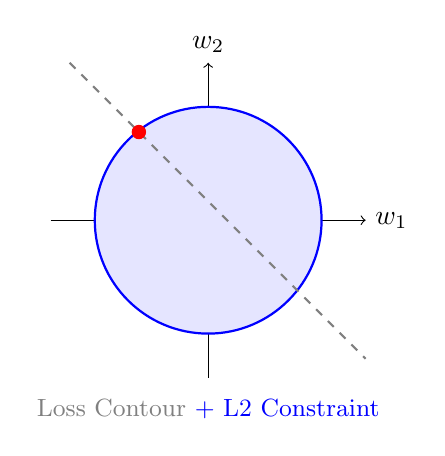
\begin{tikzpicture}[scale=0.8]
                \draw[->] (-2.5,0) -- (2.5,0) node[right] {$w_1$}; 
                \draw[->] (0,-2.5) -- (0,2.5) node[above] {$w_2$};
                \draw[blue, thick, fill=blue!10] (0,0) circle (1.8);
                \node[blue, font=\small] at (0,-3.0) {\textcolor{gray}{Loss Contour} + L2 Constraint};

                % (fix) make dashed line pass through the red point
                \draw[gray, thick, dashed] (-2.2,2.5) -- (2.5,-2.2);

                \filldraw[red] (-1.1, 1.4) circle (3pt);
            \end{tikzpicture}
            
            \vspace{0.5em}
            \small Ridge: Smooth solution, rarely hits axis \\ $w_1=-1.5, w_2=2.0$
        \end{column}
         
        \begin{column}{0.50\textwidth}
            \centering
            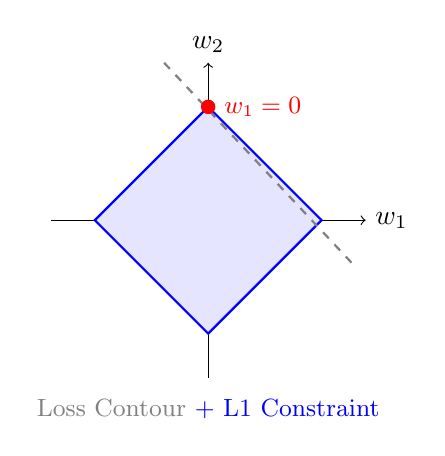
\begin{tikzpicture}[scale=0.8]
                \draw[->] (-2.5,0) -- (2.5,0) node[right] {$w_1$}; 
                \draw[->] (0,-2.5) -- (0,2.5) node[above] {$w_2$};
                \draw[blue, thick, fill=blue!10] (0,1.8) -- (1.8,0) -- (0,-1.8) -- (-1.8,0) -- cycle;
                \node[blue, font=\small] at (0,-3.0) {\textcolor{gray}{Loss Contour} + L1 Constraint};

                % (fix) make dashed line pass through the corner (red point)
                \draw[gray, thick, dashed] (-0.7,2.5) -- (2.3,-0.7);

                \filldraw[red] (0, 1.8) circle (3pt);
                \node[right, red, font=\small] at (0.1, 1.8) {$w_1=0$};
            \end{tikzpicture}
            
            \vspace{0.5em}
            \small Lasso: Sharp corners promote sparsity \\ $w_1=0, w_2=2.5$
        \end{column}
    \end{columns}
\end{frame}

% =================================================================
% 3. LOGISTIC REGRESSION
% =================================================================
% \section{3. Logistic Regression}

% --- Slide 1: The Challenge ---
